\documentclass[%
12pt,
master,  % тип документа
natbib,      % использовать пакет natbib для "сжатия" цитирований
subf,        % использовать пакет subcaption для вложенной нумерации рисунков
substylefile = spbu.rtx,
href,        % использовать пакет hyperref для создания гиперссылок
colorlinks,  % цветные гиперссылки
%fixint,     % включить прямые знаки интегралов
]{disser}

\usepackage[
  a4paper, mag=1000,
  left=2.5cm, right=1cm, top=2cm, bottom=2cm, headsep=0.7cm, footskip=1cm
]{geometry}


\usepackage[colorinlistoftodos]{todonotes}

\usepackage[intlimits]{amsmath}
\usepackage{amssymb,amsfonts}

\usepackage[T2A]{fontenc}
\usepackage[utf8]{inputenc}
%\usepackage[cp1251]{inputenc}
\usepackage[english,russian]{babel}
%\usepackage[backend = biber]{biblatex}
\ifpdf\usepackage{epstopdf}\fi
\usepackage[autostyle]{csquotes}
\bibliographystyle{utf8gost705u}
%\bibliographystyle{gost2008}
%\usepackage[backend=biber, babel=other, style=gost-authoryear]{biblatex}
%\bibliographystyle{gost780s}

% Шрифт Times в тексте как основной
%\usepackage{tempora}
% альтернативный пакет из дистрибутива TeX Live
%\usepackage{cyrtimes}

% Шрифт Times в формулах как основной
%\usepackage[varg,cmbraces,cmintegrals]{newtxmath}
% альтернативный пакет
%\usepackage[subscriptcorrection,nofontinfo]{mtpro2}

% Плавающие рисунки "в оборку".
\usepackage{wrapfig}

% Номера страниц снизу и по центру
%\pagestyle{footcenter}
%\chapterpagestyle{footcenter}

% Точка с запятой в качестве разделителя между номерами цитирований
%\setcitestyle{semicolon}

% Использовать полужирное начертание для векторов
\let\vec=\mathbf

% Включать подсекции в оглавление
\setcounter{tocdepth}{2}

\graphicspath{{fig/}}

\begin{document}
% Переопределение стандартных заголовков
%\def\contentsname{Содержание}
%\def\conclusionname{Выводы}
%\def\bibname{Литература}

%
% Титульный лист на русском языке
%

\institution{%
	Санкт-Петербургский государственный университет \\
	Прикладная математика и информатика \\
	Статистическое моделирование
}

% Имя лица, допускающего к защите (зав. кафедрой)
% \apname{ФИО зав. кафедрой}

\title{Отчет о научно-исследовательской работе}

\topic{\normalfont\scshape%
	Обнаружение разладки во временных рядах показов мобильной
рекламы}

% Автор
\author{Мерзляков Климент Викторович}
% Группа
\group{Студента группы 17.М03-мм}

% Научный руководитель
\sa {Н.\,Э.~Голяндина}
\sastatus{к.\,ф.-м.\,н., доцент}


% Рецензент
% \rev      {П.\,П.~Петров}
% \revstatus{к.\,ф.-м.\,н., доцент}

% Город и год
\city{Санкт-Петербург}
\date{\number\year}

\maketitle

%%
%% Titlepage in English
%%
%
%\setlength\thirdskip{0pt}
%
%\institution{Name of Organization}
%
%% Approved by
%\apname{Professor S.\,S.~Sidorov}
%
%\title{Diploma Thesis}
%
%% Topic
%\topic{Dummy Title}
%
%% Author
%\author{Author's Name} % Full Name
%\group{} % Study Group
%
%% Scientific Advisor
%\sa       {I.\,I.~Ivanov}
%\sastatus {Professor}
%
%% Reviewer
%\rev      {P.\,P.~Petrov}
%\revstatus{Associate Professor}
%
%% Consultant
%\con{}
%\conspec{}
%\constatus{}
%
%% City & Year
%\city{Saint Petersburg}
%\date{\number\year}
%
%\maketitle[en]

% Содержание
\tableofcontents

% Введение
% \input{intro}

\nocite{*}



\intro

Рекламной сетью называют некоторую площадку или систему, которая является посредником между рекламодателями и собственниками рекламных мест --- владельцев сайтов, мобильных приложений и каких-либо других пространств, где можно размещать рекламу.

В интернет-рекламе взаимодействие рекламной сети с пользователем можно описать следующей последовательностью событий. При выполнении некоторых условий (например, пользователь открыл мобильное приложение) с устройства пользователя отправляется запрос на показ рекламы. Если запрос удовлетворяется, то происходит событие „показ“, то есть пользователь непосредственно видит рекламу. После этого может произойти событие „клик“ и далее какое-либо целевое действие. В мобильной интернет-рекламе „показ“ является одним из ключевых событий, поскольку он отражает количество рекламы доставленное до конечного пользователя.

Рекламные интернет-сети являются интересным объектом для исследования с точки зрения обнаружения разладки, поскольку все показатели отслеживаются с точностью до секунды, происходит большое количество событий, а так как рекламные сети, как правило, работают на международном рынке, то существует возможность тестировать гипотезы на большом количестве различных временных рядов.

Одной из текущих проблем, стоящих перед рекламными сетями --- это низкая скорость реагирования на любые резкие изменения текущего состояния. Такие изменения отражаются в данных в виде аномальных значений, резких всплесков и внезапных изменений тренда. Проблема заключается в том, что показателей требующих отслеживания могут быть десятки, при этом на каждый показатель может влиять большое количество факторов. Поэтому зачастую, чтобы локализовать и устранить проблему, требуется просмотреть сотни графиков. Отсюда следует, что наличие качественного метода обнаружения разладки каждого показателя по каждому измерению позволило бы не только существенно сэкономить ресурсы, но и в целом повысить эффективность бизнеса. Поэтому целью данной работы является разработка методики обнаружения разладки. В работе будут использоваться фактические, данные одной из работающих рекламных сетей.



% Глава 2
\chapter{Обнаружение разладки во временных рядах}

\section{Построение модели данных}\label{section:data_modeling}

Реальные данные интернет-рекламы имеют стабильную дневную периодичность (на рисунке ~\ref{fig:examples_day} приведен пример типичной динамики в рамках дня). По более длинному ряду, изображенному на рисунке ~\ref{fig:examples_month}, видно, что в данных время от времени возникают разладки разных видов, при этом сам ряд имеет мультипликативный характер (с изменением среднего уровня ряда пропорционально меняется и амплитуда колебаний). В реальных временных рядах достаточно сложно разметить наличие разладок --- зачастую сложно отделить разладку от шума. Поэтому вместо разметки реальных рядов мы будем моделировать искусственные ряды, похожие на ряды данных интернет-рекламы с определенным шумом и разладками в известных местах.

\begin{figure}[!hhh]
	\begin{center}
		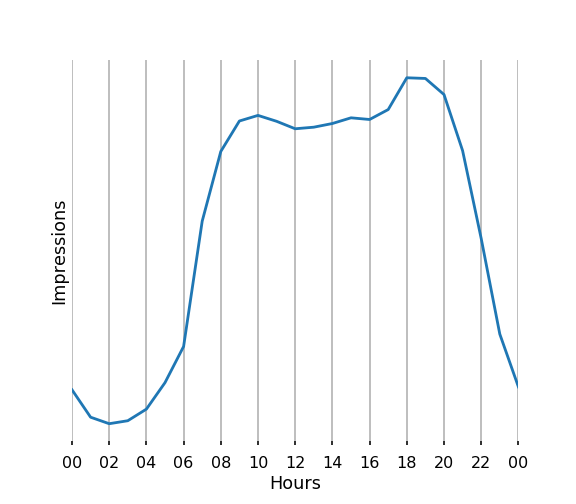
\includegraphics[width=12cm]{examples_day}
	\end{center}
	\vspace{-5mm}\caption{Пример количества показов рекламы за сутки}
	\label{fig:examples_day}
\end{figure}
 
\begin{figure}[!hhh]
	\begin{center}
		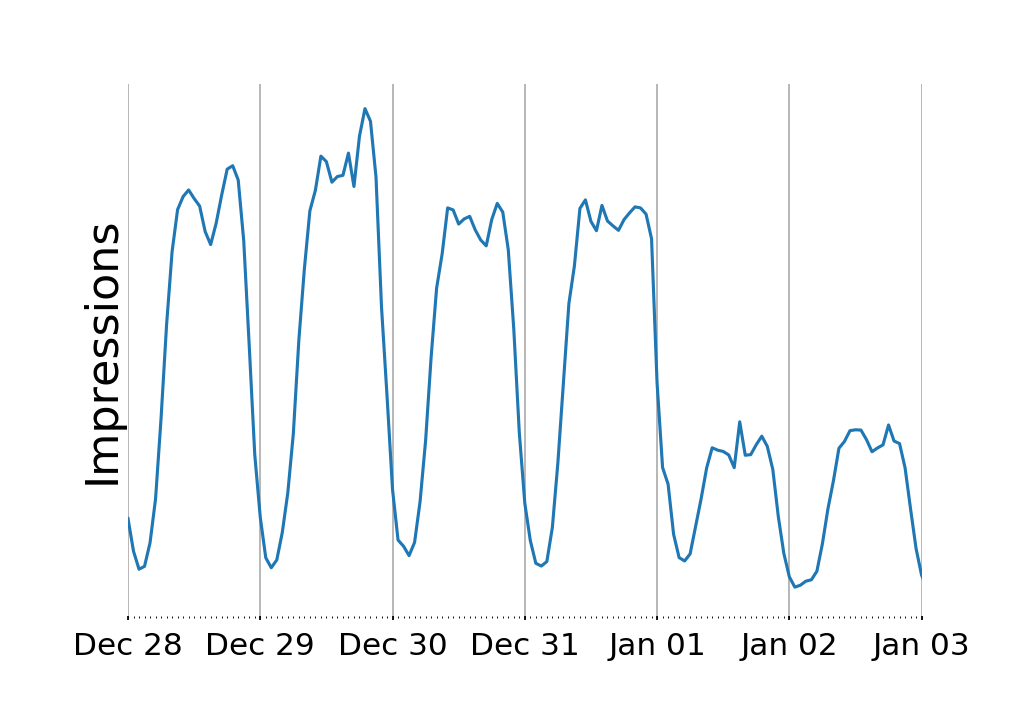
\includegraphics[width=12cm]{cp_mean_2}
	\end{center}
	\vspace{-5mm}\caption{Пример количества показов рекламы с разладкой за неделю}
	\label{fig:examples_month}
\end{figure}

Обозначим временной ряд $Y = (y_1, \dots, y_n)$. Наблюдаемые значения ряда можно представить в виде суммы компонент:
\begin{equation*}
Y = T + S + E ,
\end{equation*}
где  $ T = (t_1, \dots, t_n) $ компонента-тренд, $ S = (s_1, \dots, s_n) $ периодическая компонента, $ E = (\epsilon_1, \dots, \epsilon_n) $ остатки или шум.
Для каждой из этих компонент требуется построить модель. Это можно сделать, например, следующим образом:
\begin{equation*}
t_i = c, \quad i = 1, \dots, n, 
\end{equation*}

\begin{equation*}
s_i = A \cos \left( \frac{2\pi}{a} i + \phi \right), \quad i = 1, \dots, n,
\end{equation*}

\begin{equation*}
\epsilon_i \sim N(\mu, \sigma^2), \quad i = 1, \dots, n, 
\end{equation*}
где $i$ индекс элемента ряда; $c$ --- константа, $A$ --- амплитуда; $a$ --- период; $\phi$ --- фаза.

Ряды, модель которых мы хотим построить, имеют мультипликативность (амплитуда колебаний меняется пропорционально изменению тренда). Такого эффекта можно достичь, взяв экспоненту от исходной модели ряда:
\begin{equation*}
Y^{\mathrm{(mult)}} = e^{Y}. 
\end{equation*}

Построим модель разладки, исходя из следующего:
\begin{itemize}
	\item Разладка только в одной точке ряда;
	\item Разладка только в тренде и заключается в сдвиге;
	\item Разладка может произойти не всегда, а с некоторой вероятностью $\rho$.
\end{itemize}
Формально это можно описать так: пусть $\tau$ --- точка (индекс) разладки, тогда тренд с разладкой обозначим $ \tilde{T} = (\tilde{t_1}, \dots, \tilde{t_n}) $, где
\begin{equation*}
\tilde{t_i} =
	\begin{cases}
		t_i, & i < \tau, \\
		t_i + \delta, & i \geqslant \tau,
	\end{cases}
\end{equation*}

$ \delta $  --- значение разладки.

Значение разладки является случайной величиной с некоторым распределением. В данной работе значение разладки будет иметь нормальное распределение $ \delta^* \sim N(\mu^{\mathrm{(cp)}}, \sigma^{2\mathrm{(cp)}})  $, с некоторой вероятностью возникновения $ \rho $:

\begin{equation*}
\delta = \begin{cases}
    		\delta^*, & \textrm{с вероятностью } \rho, \\
  		0, & \textrm{с вероятностью } 1 - \rho.
	\end{cases} 
\end{equation*}

Таким образом, $\delta$ является случайной величиной с распределением-смесью. При этом точка разладки  $\tau$ тоже является случайной величиной с равномерным распределением на $ [n_0, \dots, n - n_0 ] $, где $ n_0 $ --- самая первая возможная точка разладки, которая задается параметром. $n_0$ введена намеренно, чтобы разладка при моделировании не возникала в первых и последних точках ряда.

Таким образом, моделируемый ряд с разладкой будет иметь следующий вид:
%\begin{equation*} Y = e^{\tilde{T} + S + E}.  \end{equation*}
\begin{equation*}
\tilde{Y}^{\mathrm{(mult)}} = e^{\tilde{T} + S + E}. 
\end{equation*}

В результате модель временного ряда имеет пять параметров: $ A, a, \phi, \mu, \sigma, c $, а модель разладки имеет еще четыре параметра: $ \mu^{\mathrm{(cp)}}, \sigma^{\mathrm{(cp)}}, \rho, n_0 $.

\section{Методы обнаружения разладки}


Опишем один из подходов к обнаружению разладки. Данный подход не является единственным, хотя заключает в себе широкое разнообразие методов. Как правило, у временного ряда есть некоторая структура (сигнал), которая может быть описана той или иной моделью. Идея подхода заключается в том, что около точки разладки модель плохо описывает временной ряд. Используя некоторую меру ошибки мы можем измерять то, насколько хорошо или плохо описывает выбранная модель реальные данные. Как только ошибка (отклонение модели от реальных данных) превышает заданный порог, метод сигнализирует о разладке.

Можно выделить два типа методов в данном подходе:
\begin{itemize}
	\item Методы на основе предсказания
	\item Методы на основе аппроксимации
\end{itemize}

\subsection{Методы на основе аппроксимации}

Пусть $l$ --- чётное вещественное число, называемое шириной окна. При этом  $ 1 < l < n $. С помощью ширины окна из исходного ряда образуется последовательность подрядов $W = \{ w_j \}_{j=1}^k$, где $k = n - l + 1$ --- количество таких подрядов; а $ w_j = (y_j, \dots, y_{j+l-1}) $ --- $j$-ый подряд. Каждый подряд  $w_j$  в свою очередь делится на два подряда одинаковой длины (это возможно, поскольку $l$ четное по условию): $ W^{\mathrm{(left)}} = \{w_j^{\mathrm{(left)}} \}  =  \{(y_j, \dots, y_{j+\frac{l}{2}-1}) \}$ и $W^{\mathrm{(right)}} = \{w_j^{\mathrm{(right)}} \} = \{(y_{j+\frac{l}{2}}, \dots, y_{j+l-1}) \}$.

Таким образом, для каждого ряда $W$ можно сформировать тройки рядов: 

\begin{equation*}
W^{\mathrm{(all)}} = \{w_j^{\mathrm{(all)}} \}_{j=1}^k =  \{(w_j; w_j^{\mathrm{(left)}}; w_j^{\mathrm{(right)}}) \}_{j=1}^k. 
\end{equation*}

Пусть есть функция ошибки $e(\cdot)$, такая что:
\begin{equation*}
e(X) = \min_{\theta}{\sum_{p=1}^m(x_p - f(x_p | \theta))^2 },
\end{equation*}
где $X = (x_1, \dots, x_m)$ ---  вещественный временной ряд длины $m$, а $f(x | \theta)$ --- модель сигнала этого временного ряда с параметрами $\theta$.

Функция $f(x|\theta)$ может быть константной ($\theta = (b)$):
\begin{equation*}
f(x | b) = b,
\end{equation*}
либо другой подходящей под наш ряд функцией, например:
\begin{equation*}
f(x | P, p, \chi) = P\cos(\frac{2\pi}{p}x + \chi) + b. 
\end{equation*}

Мера ошибки позволяет нам рассчитать, насколько хорошо аппроксимируется отрезок ряда с помощью выбранной модели. Однако, для обнаружения самой разладки необходимо еще ввести функцию разладки:
\begin{equation*}
F(w_j^{\mathrm{(all)}} ) = \frac{e(w_j) - e(w_j^{\mathrm{(left)}}) - e(w_j^{\mathrm{(right)}})}{h}, 
\end{equation*}
где $h$ --- значение нормировки, $j = 1, \dots, k$.

Отметим, что значения функции разладки синхронизируются с исходным рядом по последнему индексу окна. То есть $F(w_1^{\mathrm{(all)}}) $ соответствует $y_l$, а $F(w_k^{\mathrm{(all)}}) $ соответсвует $y_n$.

Расчет нормирующей константы является открытой проблемой, поскольку имеются разные варианты её расчета со своими плюсами и минусами.
Например, можно рассчитывать её как значение функции ошибки на первом отрезке ряда (предполагая, что на этом отрезке не происходило разладок):
\begin{equation*} 
h = F(w_1^{\mathrm{(all)}}) = e(w_1) - e(w_1^{\mathrm{(left)}}) - e(w_1^{\mathrm{(right)}}). 
\end{equation*}

Для наглядности, на рисунке ~\ref{fig:approximation_example_1} приведен пример расчета ошибки на одном левом ряде $ w_j^{\mathrm{(left)}} $ и на одном правом ряде $ w_j^{\mathrm{(right)}} $. А на рисунке ~\ref{fig:approximation_example_2} показан пример расчет ошибки на одном общем ряде (в который входит и левая и правая части).


\begin{figure}[!hhh]
	\begin{center}
		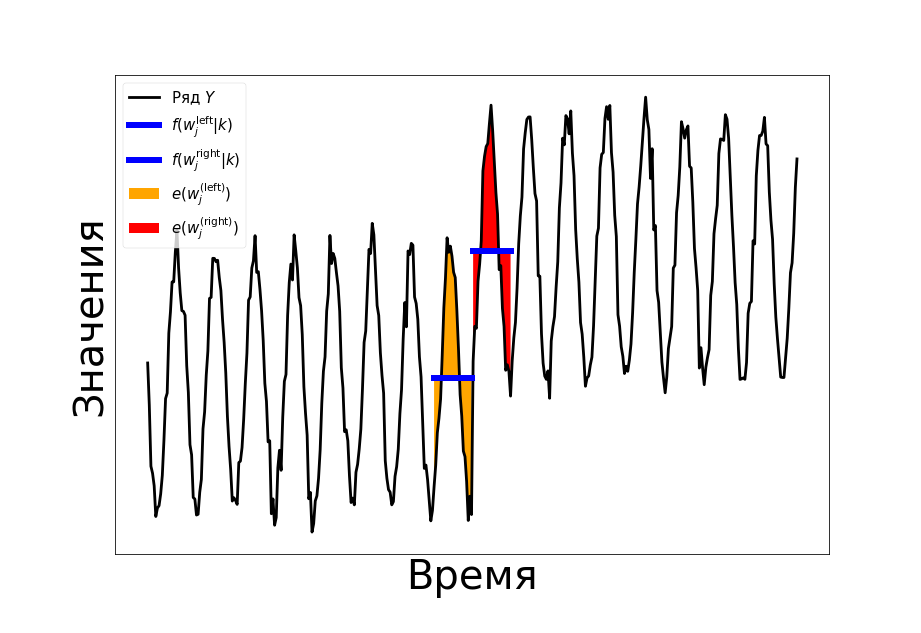
\includegraphics[width=12cm]{approaches_second_2_ru}
	\end{center}
	\vspace{-5mm}\caption{Пример промежуточного расчета ошибки методом аппроксимации}
	\label{fig:approximation_example_1}
\end{figure}

\begin{figure}[!hhh]
	\begin{center}
		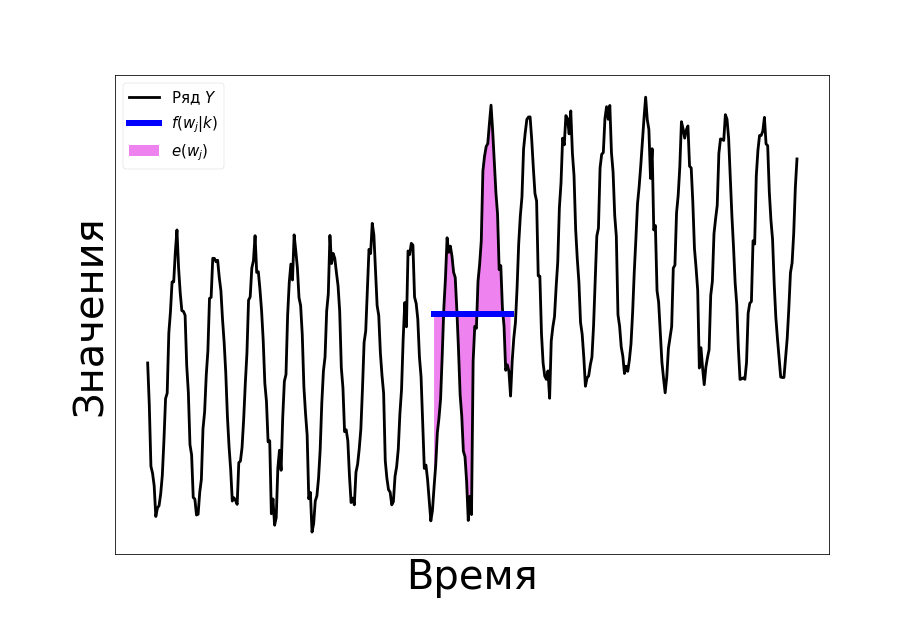
\includegraphics[width=12cm]{approaches_second_3_ru}
	\end{center}
	\vspace{-5mm}\caption{Пример промежуточного расчета ошибки методом аппроксимации, продолжение.}
	\label{fig:approximation_example_2}
\end{figure}


Итого, взяв ряд $Y$, мы «скользим» по нему окном ширины $l$ и рассчитываем значения функции разладки $F()$ для каждого из получаемых подрядов $W^{\mathrm{(all)}}$. Функция разладки начинает расти в окрестности точки разладки $\tau$, следовательно можно задать некий порог $\gamma$, такой что при превышении функции разладки этого порога в какой-то точке $\hat{\tau}$ будем считать, что разладка обнаружена в этой точке.

В результате, в данных методах нужно задавать следующие параметры: ширину окна $l$, модель $f$ и порог $\gamma$.

\subsection{Методы на основе прогнозирования}

Методы на основе прогнозирования очень похожи на методы с использованием аппроксимации. Суть их заключается в том, что мы строим прогноз на несколько точек ряда вперед и считаем отклонение фактических значений от прогнозных. В случае, если отклонение выше заданного порога, метод обнаруживает разладку.
Формально, оставаясь в тех же обозначениях, есть всё та же ширина окна $l$ (однако $l$ в данном случае может быть нечетным) и последовательность подрядов $W = \{ w_j \}_{j=1}^k$. Каждый подряд  $w_j$ делится в этом методе на два ряда не обязательно одинаковой длины. Введем индекс $g$, который будет указывать в какой точке ряда $w_j$ он будет разделен на два. Таким образом, формируется набор из пар рядов:  $ W^{\mathrm{(left)}} = \{w_j^{\mathrm{(left)}} \}  =  (y_j, \dots, y_{j+g})$ и $W^{\mathrm{(right)}} = \{w_j^{\mathrm{(right)}} \} = (y_{j+g}, \dots, y_{j+l})$. Ключевое отличие от методов аппроксимации заключается в том, что вместо расчета меры ошибки на том же ряду на котором подбирались параметры модели, мы оцениваем параметры $\theta$ модели $f(x|\theta)$ на ряде $ w_j^{\mathrm{(left)}} $, делаем прогноз на $ l - g $ точек и рассчитываем функцию ошибки $ e(\cdot) $ на ряде $ w_j^{\mathrm{(right)}} $. При этом функция разладки принимает следующий вид:
	\begin{equation*}
	 F(W^{\mathrm{(right)}}) = \frac{e(W^{\mathrm{(right)}})}{h}.
	 \end{equation*}

В остальном данные методы ничем не отличаются от методов на основе аппроксимации.

Для наглядности, на рисунке ~\ref{fig:predicition_example_1} приведен пример расчета ошибки с помощью метода прогнозирования на одном ряде  $ w_j^{\mathrm{(right)}} $. А на рисунке ~\ref{fig:predicition_example_2} показан пример расчета функции разладки $ F(W^{\mathrm{(right)}}) $ для всего ряда.

\begin{figure}[!hhh]
	\begin{center}
		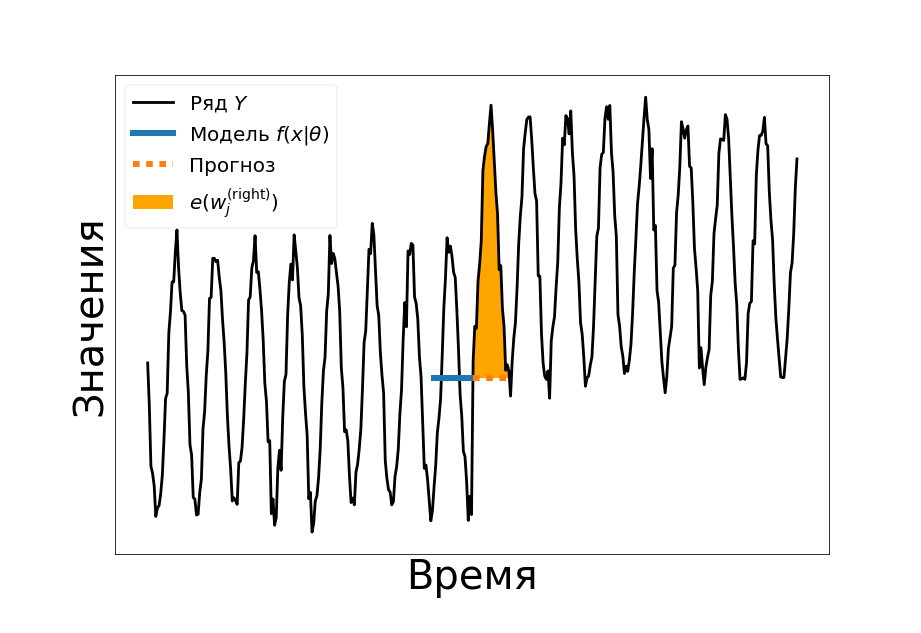
\includegraphics[width=12cm]{approaches_first_4_ru}
	\end{center}
	\vspace{-5mm}\caption{Пример расчета ошибки методом прогнозирования}
	\label{fig:predicition_example_1}
\end{figure}

\begin{figure}[!hhh]
	\begin{center}
		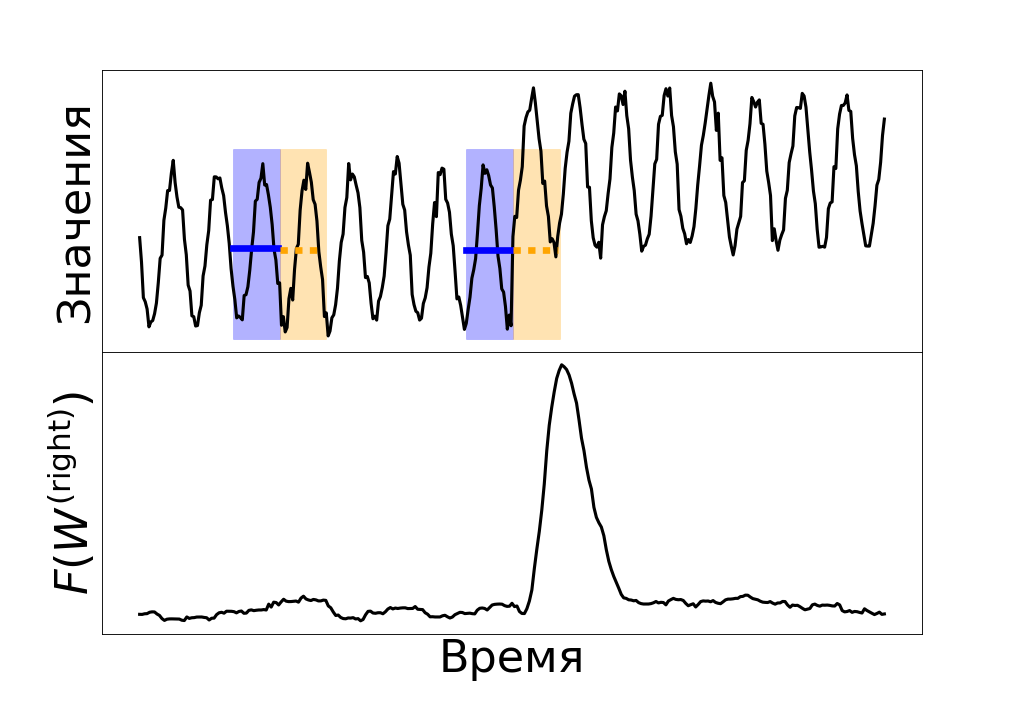
\includegraphics[width=12cm]{approaches_first_6_ru}
	\end{center}
	\vspace{-5mm}\caption{Пример расчета функции разладки с помощью скользящего окна}
	\label{fig:predicition_example_2}
\end{figure}

В методах прогнозирования нужно задавать следующие параметры: ширину окна $l$, модель $f$, индекс разделения окна (по сути с помощью него определяется на основе какого количества точек подбираются параметры модели, а на сколько точек происходит прогноз) $g$ и порог $\gamma$.


%\todo[inline]{Есть смысл в дальнейшем переписать аппроксимацию (l не обязательно четное, а функции ошибок делятся на ширину. Тогда получится универсальная запись для прогнозирования и для аппроксимации)}

\section{Оценка качества}

В рамках данной работы мы разрабатываем систему своевременного оповещения о разладках во временных рядах. При такой постановке задачи важны две характеристики: точность обнаружения разладки и скорость обнаружения разладки. Поскольку мы используем моделированные данные, то мы точно знаем в каких из смоделированных нами рядов произошла разладка, а в каких разладки не было. Более того, мы точно знаем момент разладки. Благодаря этому, мы можем строить матрицы сопряжённости и считать метрики качества. При этом важно обнаружить разладку не позднее какого-то срока, иначе оповещение о разладке будет несвоевременным. 
%Также, чтобы получать разумные результаты оценки методов, мы будем исходить из того, что метод может обнаруживать сколь угодно много разладок, в то время как фактическая разладка будет происходить только в одном месте (либо не происходить вовсе). Такая поправка введена намерено, в частности во избежания случаев, когда метод с низким значением порога $\gamma$ будет останавливаться практически сразу, из-за чего матрицы сопряженности становится проблематично интерпретировать.

% Таким образом, после каждого применения метода обнаружения разладки мы получаем вектор точек разладок $ \mathrm{\hat{T}} = (\hat{\tau}_1, \cdots, \hat{\tau}_q) $, где $q$ --- количество разладок, обнаруженное методом. Стоит отметить, что $q$ может быть равно нулю.

Исходя из этого возможны четыре варианта:

%\begin{itemize}
%	\item Разладка произошла и метод обнаружил точку разладки \textbf{после} фактической точки $\tau$, но не слишком поздно, то есть не позднее, чем $\tau + u$, где $u$ параметр. Параметром $u$ мы задаем приемлемую для нас задержку в обнаружении разладки. Такая ситуация попадает под категорию True positive.
%	\item Разладка произошла и метод не обнаружил точку разладки в диапазоне $(\tau, \cdots, \tau + u)$. Это случай False negative.
%	\item Метод обнаружил разладку там, где ее не было. То есть либо за пределами $(\tau, \cdots, \tau + u)$, либо когда разладки вообще не было в ряде. Это ситуация False positive.
%	\item Разладки не было и метод не обнаружил разладку. Это случай True negative.
%\end{itemize}

\begin{itemize}
	\item Разладка произошла и метод обнаружил точку разладки \textbf{после} фактической точки $\tau$, но не слишком поздно, то есть не позднее, чем $\tau + u$, где $u$ параметр. Параметром $u$ мы задаем приемлемую для нас задержку в обнаружении разладки. Такая ситуация попадает под категорию True positive.
	\item Разладка произошла и метод не обнаружил точку разладки в диапазоне $(\tau, \cdots, \tau + u)$. Это случай False negative.
	\item Метод обнаружил разладку в ряде без разладки. Это ситуация False positive.
	\item Разладки не было и метод не обнаружил разладку. Это случай True negative.
\end{itemize}

Договорившись о таком способе оценки качества, можно строить ROC-кривые (изменяя порог $\gamma$) для разных методов обнаружения разладки, сравнивая как работают те или иные методы в контролируемой среде эксперимента.


\chapter{Численные эксперименты}


\section{Моделирование данных}

На рисунке ~\ref{fig:examples_month} представлен пример реальных почасовых данных за семь дней. Существенно упрощая, мы можем смоделировать данный ряд используя подход, описанный в разделе ~\ref{section:data_modeling}. Для простоты дальнейшей работы зафиксируем длину ряда $n = 400$. Значение тренда пока что выберем нулевым: $c = 0$, то есть $t_i = 0, i = 1,\cdots, n$; амплитуду колебаний $A = 1$; период $ a = 24 $ (поскольку реальные данные имеют очевидную суточную периодичность); фазу $\phi = \frac{\pi}{2}$; параметры шума $\mu = 0, \sigma = 0.2$.

Таким образом, модель для генерации ряда имеет следующий вид:
\begin{equation*} y_i = \cos \left( \frac{2\pi}{24}i + \frac{\pi}{2} \right) + N(0,0.2).\end{equation*}

Пример сгенерированного ряда показан на рисунке ~\ref{fig:data_modeling_example_1}.

\begin{figure}[!hhh]
	\begin{center}
		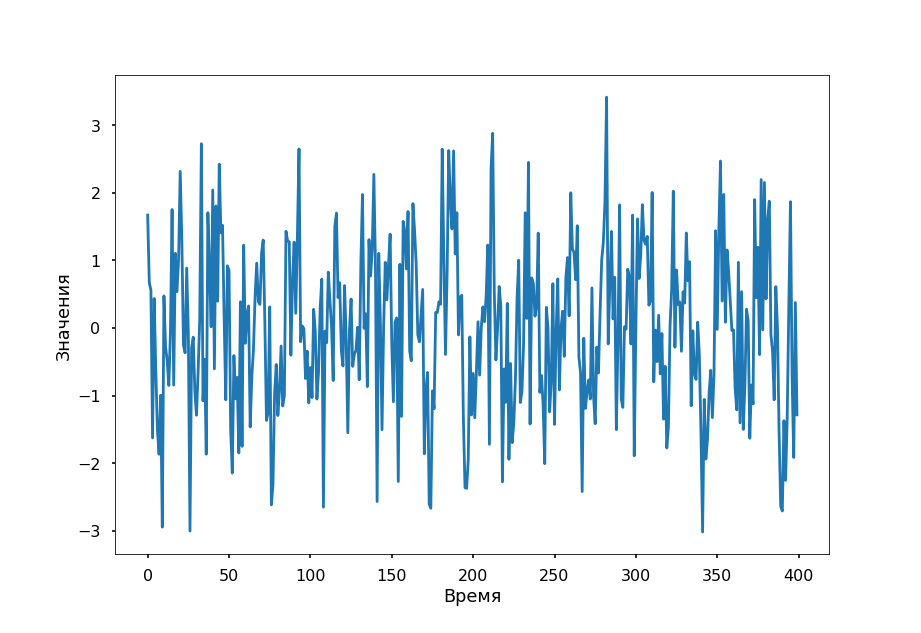
\includegraphics[width=12cm]{data_modeling_example_1}
	\end{center}
	\vspace{-5mm}\caption{Пример сгенерированного ряда без разладки}
	\label{fig:data_modeling_example_1}
\end{figure}

Вероятность возникновения разладки выберем $\rho = 0.8$; величину разладки $\delta^* \sim N(\mu = 1,\sigma = 0.4)$; а отступ с обеих сторон ряда, где разладка не может возникать $n_0 = 48$.

Пример сгенерированного ряда с разладкой показан на рисунке ~\ref{fig:data_modeling_example_2}.

\begin{figure}[!hhh]
	\begin{center}
		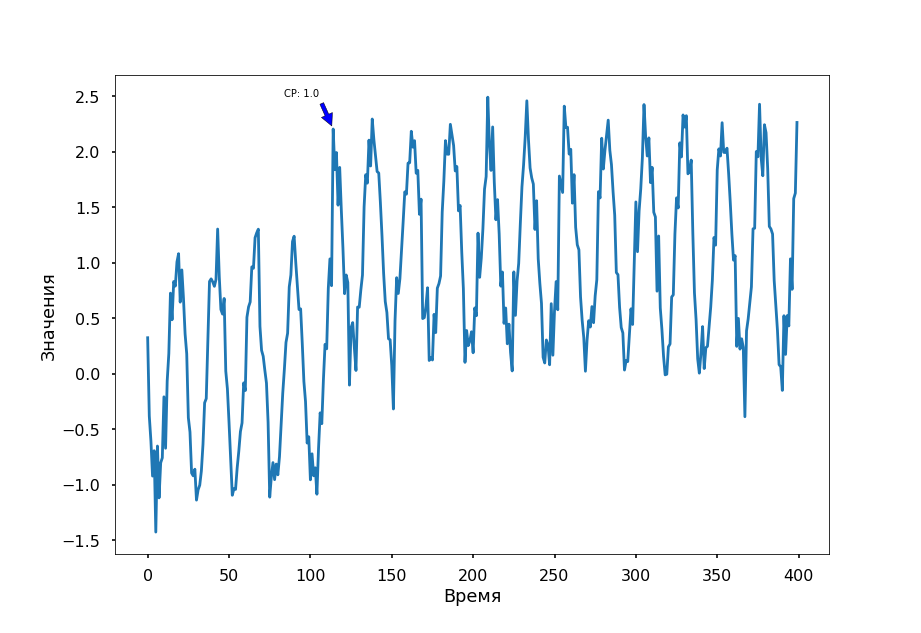
\includegraphics[width=12cm]{data_modeling_example_2}
	\end{center}
	\vspace{-5mm}\caption{Пример сгенерированного ряда с разладкой}
	\label{fig:data_modeling_example_2}
\end{figure}

 Поскольку реальные данные имеют мультипликативный характер, то мы будем брать экспоненту от сгенерированных с разладкой рядов. На рисунке ~\ref{fig:data_modeling_example_3} показан пример того же ряда, что и на рисунке ~\ref{fig:data_modeling_example_2}, но со взятой экспонентой от ряда.

 \begin{figure}[!hhh]
	\begin{center}
		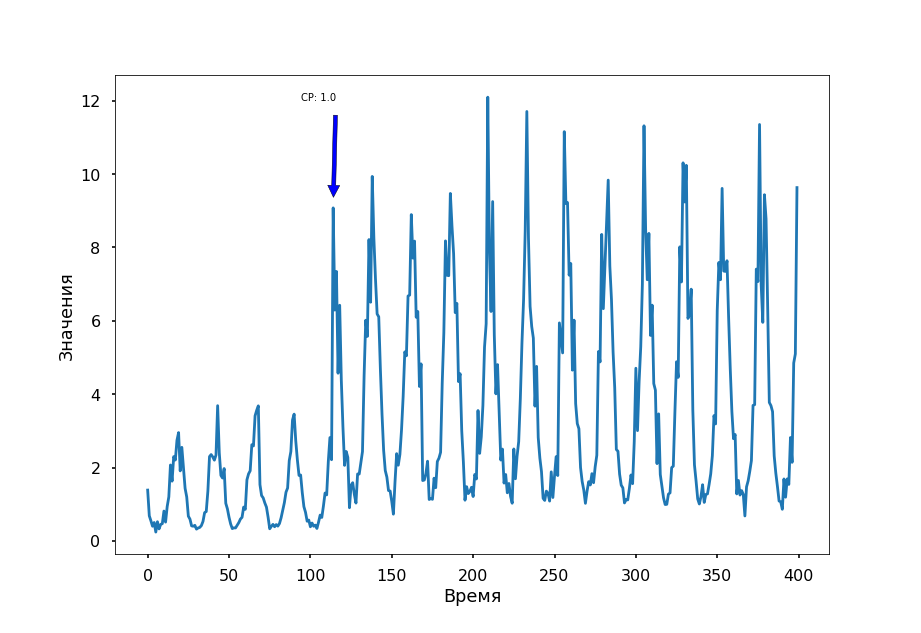
\includegraphics[width=12cm]{data_modeling_example_3}
	\end{center}
	\vspace{-5mm}\caption{Пример сгенерированного ряда с разладкой и мультипликативностью}
	\label{fig:data_modeling_example_3}
\end{figure}
%
%Как мы видим, за счет мультипликативности, в некоторых случаях ряд может слишком сильно изменяться --- вероятно нужно будет поменять некоторые параметры моделирования ряда, чтобы он стал больше похож на реальный ряд. Поэтому пока начнем с рядов без мультипликативности. В целом, результат похож на реальные ряды, поэтому пока будем двигаться дальше с такими параметрами моделирования.

%\todo[inline]{В качестве идеи на полях: можно ввести какую-то метрику схожести сгенерированных рядов и реальных.}


\section{Применение методов к моделированным данным и оценка качества этих методов}

Сгенерируем 1000 рядов со случайным местом возникновения разладки $\tau$, случайной величиной разладки $\delta$ и случайным шумом $e$ и применить к каждому из этих рядов метод обнаружения разладки на основе аппроксимации. Функцию аппроксимации возьмем константную $\theta = (b)$, ширину окна $l = 48$, а порог $\gamma$ будем брать в диапазоне от $0$ до $1$ с шагом $0.01$. Пример функции разладки для данного метода с такими параметрами изображен на рисунке  ~\ref{fig:approximation_mean_1}. При этом, в качестве приемлемой задержке возьмем $u = 48$. Это означает, нотификация с запаздыванием в двое суток является для нас приемлемой, что, разумеется, не всегда верно в реальных задачах.

\begin{figure}[!hhh]
	\begin{center}
		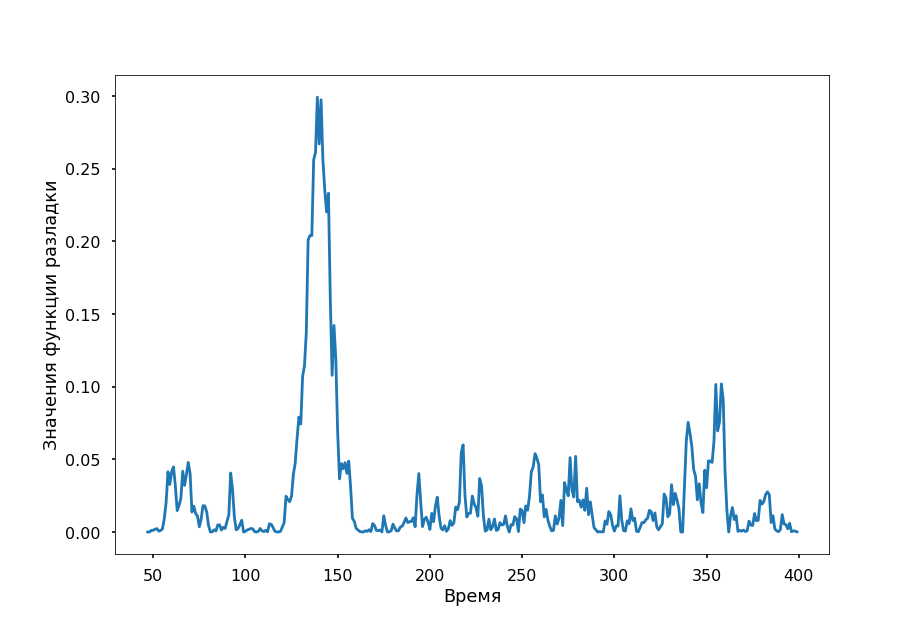
\includegraphics[width=12cm]{approximation_mean_1}
	\end{center}
	\vspace{-5mm}\caption{Пример функции разладки для сгенерированного ряда с разладкой и без мультипликативности}
	\label{fig:approximation_mean_1}
\end{figure}

Для тысячи рядов с заданными параметрами метода обнаружения разладки и заданным диапазоном порога ROC-кривая получилась следующая (рисунок ~\ref{fig:approximation_mean_2_roc}). ROC-кривая проходит довольно далеко от базовой линии, что говорит о том, что в целом метод с такими параметрами работает уже достаточно хорошо (разумеется, надо понимать, что пока что мы взяли приемлемую задержку равную 48 часам, что является очень мягкими условиями эксперимента, в сравнении с реальной жизнью). 

% Во-вторых, мы видим нетипичное для ROC-кривой поведение в верхнем правом углу: кривая уходит под базовую линию. Дело всё в том, что это происходит только в случае очень низких порогов и связано с моментом обнаружения разладки. Каждый раз после обнаружения разладки в ряде, метод начинает искать следующую разладку начиная с точки последней разладки (как бы отрезая и не учитывая данные, которые были до последней разладки). Это приводит к тому, что если разладка случайно обнаружилась (а при низком пороге это типичная ситуация) незадолго до фактической разладки, то скорее всего сама разладка не будет обнаружена. Этим объясняется почему, при очень низком пороге может быть True positive rate существенно ниже 1.


\begin{figure}[!hhh]
	\begin{center}
		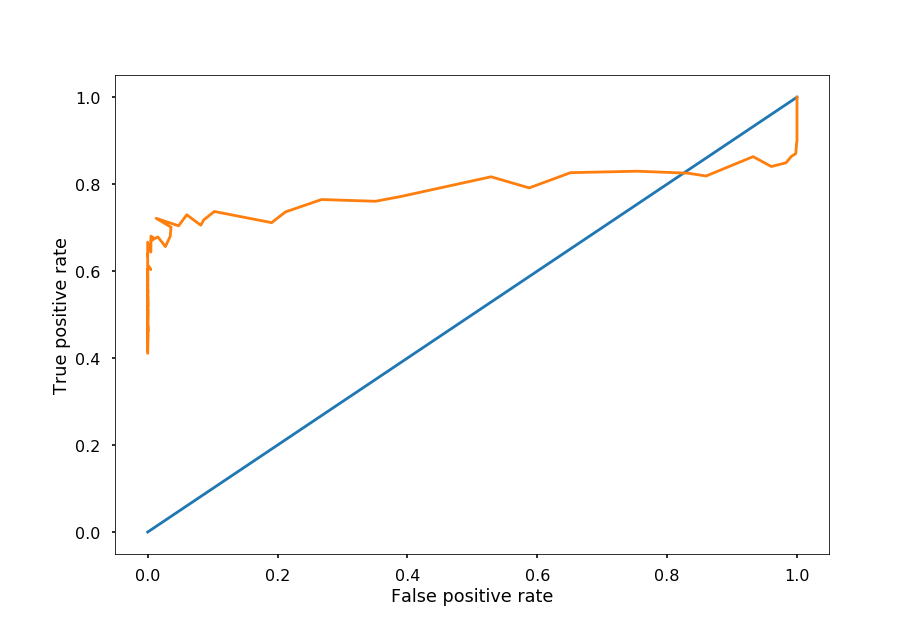
\includegraphics[width=12cm]{approximation_mean_2_roc}
	\end{center}
	\vspace{-5mm}\caption{ROC-кривая для 1000 смоделированных рядов и метода на основе аппроксимации}
	\label{fig:approximation_mean_2_roc}
\end{figure}

Попробуем применить метод обнаружения разладки на основе прогнозирования к такой же тысяче рядов. Параметры метода будем брать аналогичными параметрам аппроксимации (кроме порога). 
Функция прогнозирования константная $\theta = (b)$, ширина окна $l = 48$, индекс разделения окна $g = 24$, порог $\gamma$ будем брать в диапазоне от $0$ до $5$ с шагом $0.05$.

Получившийся результат представлен на рисунке ~\ref{fig:roc_pred_approx}. Как видно из ROC-кривых с данными параметрами метод на основе аппроксимации сработал лучше, нежели метод на основе прогнозирования. Безусловно, требуется настройка параметров, как для моделирования данных, так и для самих методов, но цель работы --- создать стенд для проверки идей и гипотез по обнаружению разладок --- достигнута, поскольку нам удалось сравнить качество двух разных методов в контролируемом эксперименте.

\begin{figure}[!hhh]
	\begin{center}
		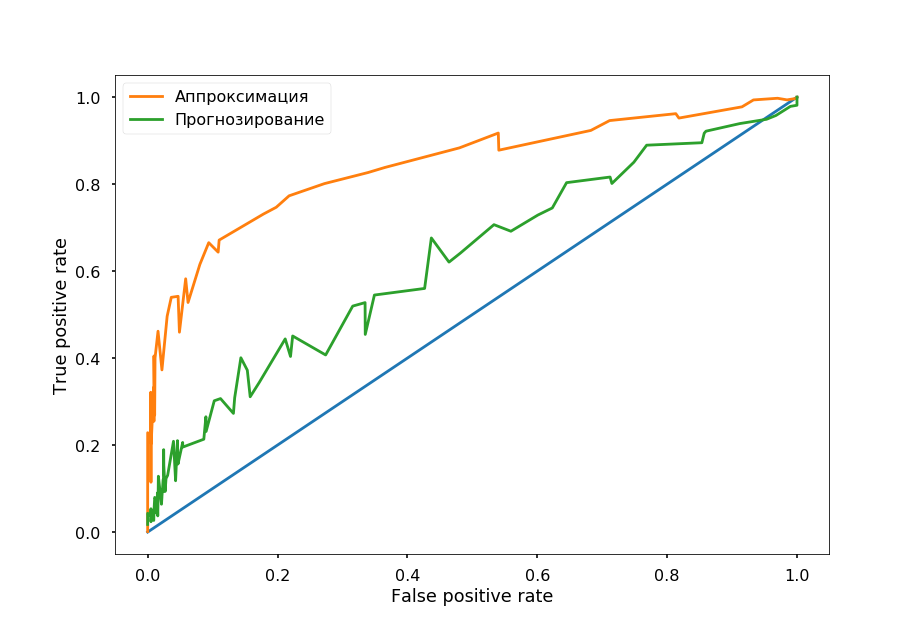
\includegraphics[width=12cm]{roc_pred_approx}
	\end{center}
	\vspace{-5mm}\caption{ROC-кривые для 1000 смоделированных рядов}
	\label{fig:roc_pred_approx}
\end{figure}


\conclusion
В данной работе мы установили подход к моделированию временных рядов данных интернет-рекламы, формально описали некоторые методы обнаружения разладки и описали способ оценки качества методов обнаружения разладки во временных рядах. Во второй части работы, мы применили описанные методы к сгенерированным данным и сравнили качество методов. Данная работа может служить платформой для дальнейших экспериментов как с точки зрения моделирования данных более похожих на реальные, так и с точки зрения оценки качества различных методов обнаружения разладки.

%\bibliography{bibliography}
\bibliography{reference}
%\bibliography{otchet}


% Не добавлять длинное тире в качестве разделителя
%\newcommand\BibDash{}
% Выделять курсивом
%\let\BibEmph=\emph
%\bibliographystyle{gost2008}

% Список литературы
% \bibliography{thesis}


%\begin{thebibliography}{9}
%	\bibitem{ssa_forecast} Голяндина Н.Э. Метод „Гусеница“-SSA: прогноз временных рядов. Учебное пособие. СПб., 2003.
%	\bibitem{armstrong} Armstrong. Principles of Forecasting: A Handbook for Researchers and Practitioners. Kluwer Academic Publishers, 2001.
%	\bibitem{dagum} Dagum, Estela, Bianconcini. Seasonal Adjustment Methods and Real Time Trend-Cycle Estimation, 2016.
%	\bibitem{ssa_book} N. Golyandina, V. Nekrutkin, A. Zhigljavsky. Analysis of Time Series Structure - SSA and Related Techniques, 2001.
%	\bibitem{hyndman} R. Hyndman, G. Athanasopoulos. Forecasting: Principles and Practice. 2013.
%	\bibitem{moving_average} R. Hyndman. Moving averages. 2009.
%	
%\end{thebibliography}

% Приложения
\appendix



\end{document}
